\documentclass[11pt]{article}
\usepackage{sectsty}
\allsectionsfont{\color{blue}\fontfamily{lmss}\selectfont}
\usepackage{fontspec}
\setmainfont{XCharter}

\usepackage{listings}
\lstset{
basicstyle=\small\ttfamily,
tabsize=8,
columns=flexible,
breaklines=true,
frame=tb,
rulecolor=\color[rgb]{0.8,0.8,0.7},
backgroundcolor=\color[rgb]{1,1,0.91},
postbreak=\raisebox{0ex}[0ex][0ex]{\ensuremath{\color{red}\hookrightarrow\space}}
}
\usepackage{fontawesome}


\usepackage{mdframed}
\newmdenv[
  backgroundcolor=gray,
  fontcolor=white,
  nobreak=true,
]{terminalinput}



\usepackage{parskip}


    \usepackage[breakable]{tcolorbox}
    \usepackage{parskip} % Stop auto-indenting (to mimic markdown behaviour)


    % Basic figure setup, for now with no caption control since it's done
    % automatically by Pandoc (which extracts ![](path) syntax from Markdown).
    \usepackage{graphicx}
    % Maintain compatibility with old templates. Remove in nbconvert 6.0
    \let\Oldincludegraphics\includegraphics
    % Ensure that by default, figures have no caption (until we provide a
    % proper Figure object with a Caption API and a way to capture that
    % in the conversion process - todo).
    \usepackage{caption}
    \DeclareCaptionFormat{nocaption}{}
    \captionsetup{format=nocaption,aboveskip=0pt,belowskip=0pt}

    \usepackage{float}
    \floatplacement{figure}{H} % forces figures to be placed at the correct location
    \usepackage{xcolor} % Allow colors to be defined
    \usepackage{enumerate} % Needed for markdown enumerations to work
    \usepackage{geometry} % Used to adjust the document margins
    \usepackage{amsmath} % Equations
    \usepackage{amssymb} % Equations
    \usepackage{textcomp} % defines textquotesingle
    % Hack from http://tex.stackexchange.com/a/47451/13684:
    \AtBeginDocument{%
        \def\PYZsq{\textquotesingle}% Upright quotes in Pygmentized code
    }
    \usepackage{upquote} % Upright quotes for verbatim code
    \usepackage{eurosym} % defines \euro

    \usepackage{iftex}
    \ifPDFTeX
        \usepackage[T1]{fontenc}
        \IfFileExists{alphabeta.sty}{
              \usepackage{alphabeta}
          }{
              \usepackage[mathletters]{ucs}
              \usepackage[utf8x]{inputenc}
          }
    \else
        \usepackage{fontspec}
        \usepackage{unicode-math}
    \fi

    \usepackage{fancyvrb} % verbatim replacement that allows latex
    \usepackage{grffile} % extends the file name processing of package graphics
                         % to support a larger range
    \makeatletter % fix for old versions of grffile with XeLaTeX
    \@ifpackagelater{grffile}{2019/11/01}
    {
      % Do nothing on new versions
    }
    {
      \def\Gread@@xetex#1{%
        \IfFileExists{"\Gin@base".bb}%
        {\Gread@eps{\Gin@base.bb}}%
        {\Gread@@xetex@aux#1}%
      }
    }
    \makeatother
    \usepackage[Export]{adjustbox} % Used to constrain images to a maximum size
    \adjustboxset{max size={0.9\linewidth}{0.9\paperheight}}

    % The hyperref package gives us a pdf with properly built
    % internal navigation ('pdf bookmarks' for the table of contents,
    % internal cross-reference links, web links for URLs, etc.)
    \usepackage{hyperref}
    % The default LaTeX title has an obnoxious amount of whitespace. By default,
    % titling removes some of it. It also provides customization options.
    \usepackage{titling}
    \usepackage{longtable} % longtable support required by pandoc >1.10
    \usepackage{booktabs}  % table support for pandoc > 1.12.2
    \usepackage{array}     % table support for pandoc >= 2.11.3
    \usepackage{calc}      % table minipage width calculation for pandoc >= 2.11.1
    \usepackage[inline]{enumitem} % IRkernel/repr support (it uses the enumerate* environment)
    \usepackage[normalem]{ulem} % ulem is needed to support strikethroughs (\sout)
                                % normalem makes italics be italics, not underlines
    \usepackage{mathrsfs}



    % Colors for the hyperref package
    \definecolor{urlcolor}{rgb}{0,.145,.698}
    \definecolor{linkcolor}{rgb}{.71,0.21,0.01}
    \definecolor{citecolor}{rgb}{.12,.54,.11}

    % ANSI colors
    \definecolor{ansi-black}{HTML}{3E424D}
    \definecolor{ansi-black-intense}{HTML}{282C36}
    \definecolor{ansi-red}{HTML}{E75C58}
    \definecolor{ansi-red-intense}{HTML}{B22B31}
    \definecolor{ansi-green}{HTML}{00A250}
    \definecolor{ansi-green-intense}{HTML}{007427}
    \definecolor{ansi-yellow}{HTML}{DDB62B}
    \definecolor{ansi-yellow-intense}{HTML}{B27D12}
    \definecolor{ansi-blue}{HTML}{208FFB}
    \definecolor{ansi-blue-intense}{HTML}{0065CA}
    \definecolor{ansi-magenta}{HTML}{D160C4}
    \definecolor{ansi-magenta-intense}{HTML}{A03196}
    \definecolor{ansi-cyan}{HTML}{60C6C8}
    \definecolor{ansi-cyan-intense}{HTML}{258F8F}
    \definecolor{ansi-white}{HTML}{C5C1B4}
    \definecolor{ansi-white-intense}{HTML}{A1A6B2}
    \definecolor{ansi-default-inverse-fg}{HTML}{FFFFFF}
    \definecolor{ansi-default-inverse-bg}{HTML}{000000}

    % common color for the border for error outputs.
    \definecolor{outerrorbackground}{HTML}{FFDFDF}

    % commands and environments needed by pandoc snippets
    % extracted from the output of `pandoc -s`
    \providecommand{\tightlist}{%
      \setlength{\itemsep}{0pt}\setlength{\parskip}{0pt}}
    \DefineVerbatimEnvironment{Highlighting}{Verbatim}{commandchars=\\\{\}}
    % Add ',fontsize=\small' for more characters per line
    \newenvironment{Shaded}{}{}
    \newcommand{\KeywordTok}[1]{\textcolor[rgb]{0.00,0.44,0.13}{\textbf{{#1}}}}
    \newcommand{\DataTypeTok}[1]{\textcolor[rgb]{0.56,0.13,0.00}{{#1}}}
    \newcommand{\DecValTok}[1]{\textcolor[rgb]{0.25,0.63,0.44}{{#1}}}
    \newcommand{\BaseNTok}[1]{\textcolor[rgb]{0.25,0.63,0.44}{{#1}}}
    \newcommand{\FloatTok}[1]{\textcolor[rgb]{0.25,0.63,0.44}{{#1}}}
    \newcommand{\CharTok}[1]{\textcolor[rgb]{0.25,0.44,0.63}{{#1}}}
    \newcommand{\StringTok}[1]{\textcolor[rgb]{0.25,0.44,0.63}{{#1}}}
    \newcommand{\CommentTok}[1]{\textcolor[rgb]{0.38,0.63,0.69}{\textit{{#1}}}}
    \newcommand{\OtherTok}[1]{\textcolor[rgb]{0.00,0.44,0.13}{{#1}}}
    \newcommand{\AlertTok}[1]{\textcolor[rgb]{1.00,0.00,0.00}{\textbf{{#1}}}}
    \newcommand{\FunctionTok}[1]{\textcolor[rgb]{0.02,0.16,0.49}{{#1}}}
    \newcommand{\RegionMarkerTok}[1]{{#1}}
    \newcommand{\ErrorTok}[1]{\textcolor[rgb]{1.00,0.00,0.00}{\textbf{{#1}}}}
    \newcommand{\NormalTok}[1]{{#1}}

    % Additional commands for more recent versions of Pandoc
    \newcommand{\ConstantTok}[1]{\textcolor[rgb]{0.53,0.00,0.00}{{#1}}}
    \newcommand{\SpecialCharTok}[1]{\textcolor[rgb]{0.25,0.44,0.63}{{#1}}}
    \newcommand{\VerbatimStringTok}[1]{\textcolor[rgb]{0.25,0.44,0.63}{{#1}}}
    \newcommand{\SpecialStringTok}[1]{\textcolor[rgb]{0.73,0.40,0.53}{{#1}}}
    \newcommand{\ImportTok}[1]{{#1}}
    \newcommand{\DocumentationTok}[1]{\textcolor[rgb]{0.73,0.13,0.13}{\textit{{#1}}}}
    \newcommand{\AnnotationTok}[1]{\textcolor[rgb]{0.38,0.63,0.69}{\textbf{\textit{{#1}}}}}
    \newcommand{\CommentVarTok}[1]{\textcolor[rgb]{0.38,0.63,0.69}{\textbf{\textit{{#1}}}}}
    \newcommand{\VariableTok}[1]{\textcolor[rgb]{0.10,0.09,0.49}{{#1}}}
    \newcommand{\ControlFlowTok}[1]{\textcolor[rgb]{0.00,0.44,0.13}{\textbf{{#1}}}}
    \newcommand{\OperatorTok}[1]{\textcolor[rgb]{0.40,0.40,0.40}{{#1}}}
    \newcommand{\BuiltInTok}[1]{{#1}}
    \newcommand{\ExtensionTok}[1]{{#1}}
    \newcommand{\PreprocessorTok}[1]{\textcolor[rgb]{0.74,0.48,0.00}{{#1}}}
    \newcommand{\AttributeTok}[1]{\textcolor[rgb]{0.49,0.56,0.16}{{#1}}}
    \newcommand{\InformationTok}[1]{\textcolor[rgb]{0.38,0.63,0.69}{\textbf{\textit{{#1}}}}}
    \newcommand{\WarningTok}[1]{\textcolor[rgb]{0.38,0.63,0.69}{\textbf{\textit{{#1}}}}}


    % Define a nice break command that doesn't care if a line doesn't already
    % exist.
    \def\br{\hspace*{\fill} \\* }
    % Math Jax compatibility definitions
    \def\gt{>}
    \def\lt{<}
    \let\Oldtex\TeX
    \let\Oldlatex\LaTeX
    \renewcommand{\TeX}{\textrm{\Oldtex}}
    \renewcommand{\LaTeX}{\textrm{\Oldlatex}}
    % Document parameters
    % Document title
    \title{index}







% Pygments definitions
\makeatletter
\def\PY@reset{\let\PY@it=\relax \let\PY@bf=\relax%
    \let\PY@ul=\relax \let\PY@tc=\relax%
    \let\PY@bc=\relax \let\PY@ff=\relax}
\def\PY@tok#1{\csname PY@tok@#1\endcsname}
\def\PY@toks#1+{\ifx\relax#1\empty\else%
    \PY@tok{#1}\expandafter\PY@toks\fi}
\def\PY@do#1{\PY@bc{\PY@tc{\PY@ul{%
    \PY@it{\PY@bf{\PY@ff{#1}}}}}}}
\def\PY#1#2{\PY@reset\PY@toks#1+\relax+\PY@do{#2}}

\@namedef{PY@tok@w}{\def\PY@tc##1{\textcolor[rgb]{0.73,0.73,0.73}{##1}}}
\@namedef{PY@tok@c}{\let\PY@it=\textit\def\PY@tc##1{\textcolor[rgb]{0.24,0.48,0.48}{##1}}}
\@namedef{PY@tok@cp}{\def\PY@tc##1{\textcolor[rgb]{0.61,0.40,0.00}{##1}}}
\@namedef{PY@tok@k}{\let\PY@bf=\textbf\def\PY@tc##1{\textcolor[rgb]{0.00,0.50,0.00}{##1}}}
\@namedef{PY@tok@kp}{\def\PY@tc##1{\textcolor[rgb]{0.00,0.50,0.00}{##1}}}
\@namedef{PY@tok@kt}{\def\PY@tc##1{\textcolor[rgb]{0.69,0.00,0.25}{##1}}}
\@namedef{PY@tok@o}{\def\PY@tc##1{\textcolor[rgb]{0.40,0.40,0.40}{##1}}}
\@namedef{PY@tok@ow}{\let\PY@bf=\textbf\def\PY@tc##1{\textcolor[rgb]{0.67,0.13,1.00}{##1}}}
\@namedef{PY@tok@nb}{\def\PY@tc##1{\textcolor[rgb]{0.00,0.50,0.00}{##1}}}
\@namedef{PY@tok@nf}{\def\PY@tc##1{\textcolor[rgb]{0.00,0.00,1.00}{##1}}}
\@namedef{PY@tok@nc}{\let\PY@bf=\textbf\def\PY@tc##1{\textcolor[rgb]{0.00,0.00,1.00}{##1}}}
\@namedef{PY@tok@nn}{\let\PY@bf=\textbf\def\PY@tc##1{\textcolor[rgb]{0.00,0.00,1.00}{##1}}}
\@namedef{PY@tok@ne}{\let\PY@bf=\textbf\def\PY@tc##1{\textcolor[rgb]{0.80,0.25,0.22}{##1}}}
\@namedef{PY@tok@nv}{\def\PY@tc##1{\textcolor[rgb]{0.10,0.09,0.49}{##1}}}
\@namedef{PY@tok@no}{\def\PY@tc##1{\textcolor[rgb]{0.53,0.00,0.00}{##1}}}
\@namedef{PY@tok@nl}{\def\PY@tc##1{\textcolor[rgb]{0.46,0.46,0.00}{##1}}}
\@namedef{PY@tok@ni}{\let\PY@bf=\textbf\def\PY@tc##1{\textcolor[rgb]{0.44,0.44,0.44}{##1}}}
\@namedef{PY@tok@na}{\def\PY@tc##1{\textcolor[rgb]{0.41,0.47,0.13}{##1}}}
\@namedef{PY@tok@nt}{\let\PY@bf=\textbf\def\PY@tc##1{\textcolor[rgb]{0.00,0.50,0.00}{##1}}}
\@namedef{PY@tok@nd}{\def\PY@tc##1{\textcolor[rgb]{0.67,0.13,1.00}{##1}}}
\@namedef{PY@tok@s}{\def\PY@tc##1{\textcolor[rgb]{0.73,0.13,0.13}{##1}}}
\@namedef{PY@tok@sd}{\let\PY@it=\textit\def\PY@tc##1{\textcolor[rgb]{0.73,0.13,0.13}{##1}}}
\@namedef{PY@tok@si}{\let\PY@bf=\textbf\def\PY@tc##1{\textcolor[rgb]{0.64,0.35,0.47}{##1}}}
\@namedef{PY@tok@se}{\let\PY@bf=\textbf\def\PY@tc##1{\textcolor[rgb]{0.67,0.36,0.12}{##1}}}
\@namedef{PY@tok@sr}{\def\PY@tc##1{\textcolor[rgb]{0.64,0.35,0.47}{##1}}}
\@namedef{PY@tok@ss}{\def\PY@tc##1{\textcolor[rgb]{0.10,0.09,0.49}{##1}}}
\@namedef{PY@tok@sx}{\def\PY@tc##1{\textcolor[rgb]{0.00,0.50,0.00}{##1}}}
\@namedef{PY@tok@m}{\def\PY@tc##1{\textcolor[rgb]{0.40,0.40,0.40}{##1}}}
\@namedef{PY@tok@gh}{\let\PY@bf=\textbf\def\PY@tc##1{\textcolor[rgb]{0.00,0.00,0.50}{##1}}}
\@namedef{PY@tok@gu}{\let\PY@bf=\textbf\def\PY@tc##1{\textcolor[rgb]{0.50,0.00,0.50}{##1}}}
\@namedef{PY@tok@gd}{\def\PY@tc##1{\textcolor[rgb]{0.63,0.00,0.00}{##1}}}
\@namedef{PY@tok@gi}{\def\PY@tc##1{\textcolor[rgb]{0.00,0.52,0.00}{##1}}}
\@namedef{PY@tok@gr}{\def\PY@tc##1{\textcolor[rgb]{0.89,0.00,0.00}{##1}}}
\@namedef{PY@tok@ge}{\let\PY@it=\textit}
\@namedef{PY@tok@gs}{\let\PY@bf=\textbf}
\@namedef{PY@tok@gp}{\let\PY@bf=\textbf\def\PY@tc##1{\textcolor[rgb]{0.00,0.00,0.50}{##1}}}
\@namedef{PY@tok@go}{\def\PY@tc##1{\textcolor[rgb]{0.44,0.44,0.44}{##1}}}
\@namedef{PY@tok@gt}{\def\PY@tc##1{\textcolor[rgb]{0.00,0.27,0.87}{##1}}}
\@namedef{PY@tok@err}{\def\PY@bc##1{{\setlength{\fboxsep}{\string -\fboxrule}\fcolorbox[rgb]{1.00,0.00,0.00}{1,1,1}{\strut ##1}}}}
\@namedef{PY@tok@kc}{\let\PY@bf=\textbf\def\PY@tc##1{\textcolor[rgb]{0.00,0.50,0.00}{##1}}}
\@namedef{PY@tok@kd}{\let\PY@bf=\textbf\def\PY@tc##1{\textcolor[rgb]{0.00,0.50,0.00}{##1}}}
\@namedef{PY@tok@kn}{\let\PY@bf=\textbf\def\PY@tc##1{\textcolor[rgb]{0.00,0.50,0.00}{##1}}}
\@namedef{PY@tok@kr}{\let\PY@bf=\textbf\def\PY@tc##1{\textcolor[rgb]{0.00,0.50,0.00}{##1}}}
\@namedef{PY@tok@bp}{\def\PY@tc##1{\textcolor[rgb]{0.00,0.50,0.00}{##1}}}
\@namedef{PY@tok@fm}{\def\PY@tc##1{\textcolor[rgb]{0.00,0.00,1.00}{##1}}}
\@namedef{PY@tok@vc}{\def\PY@tc##1{\textcolor[rgb]{0.10,0.09,0.49}{##1}}}
\@namedef{PY@tok@vg}{\def\PY@tc##1{\textcolor[rgb]{0.10,0.09,0.49}{##1}}}
\@namedef{PY@tok@vi}{\def\PY@tc##1{\textcolor[rgb]{0.10,0.09,0.49}{##1}}}
\@namedef{PY@tok@vm}{\def\PY@tc##1{\textcolor[rgb]{0.10,0.09,0.49}{##1}}}
\@namedef{PY@tok@sa}{\def\PY@tc##1{\textcolor[rgb]{0.73,0.13,0.13}{##1}}}
\@namedef{PY@tok@sb}{\def\PY@tc##1{\textcolor[rgb]{0.73,0.13,0.13}{##1}}}
\@namedef{PY@tok@sc}{\def\PY@tc##1{\textcolor[rgb]{0.73,0.13,0.13}{##1}}}
\@namedef{PY@tok@dl}{\def\PY@tc##1{\textcolor[rgb]{0.73,0.13,0.13}{##1}}}
\@namedef{PY@tok@s2}{\def\PY@tc##1{\textcolor[rgb]{0.73,0.13,0.13}{##1}}}
\@namedef{PY@tok@sh}{\def\PY@tc##1{\textcolor[rgb]{0.73,0.13,0.13}{##1}}}
\@namedef{PY@tok@s1}{\def\PY@tc##1{\textcolor[rgb]{0.73,0.13,0.13}{##1}}}
\@namedef{PY@tok@mb}{\def\PY@tc##1{\textcolor[rgb]{0.40,0.40,0.40}{##1}}}
\@namedef{PY@tok@mf}{\def\PY@tc##1{\textcolor[rgb]{0.40,0.40,0.40}{##1}}}
\@namedef{PY@tok@mh}{\def\PY@tc##1{\textcolor[rgb]{0.40,0.40,0.40}{##1}}}
\@namedef{PY@tok@mi}{\def\PY@tc##1{\textcolor[rgb]{0.40,0.40,0.40}{##1}}}
\@namedef{PY@tok@il}{\def\PY@tc##1{\textcolor[rgb]{0.40,0.40,0.40}{##1}}}
\@namedef{PY@tok@mo}{\def\PY@tc##1{\textcolor[rgb]{0.40,0.40,0.40}{##1}}}
\@namedef{PY@tok@ch}{\let\PY@it=\textit\def\PY@tc##1{\textcolor[rgb]{0.24,0.48,0.48}{##1}}}
\@namedef{PY@tok@cm}{\let\PY@it=\textit\def\PY@tc##1{\textcolor[rgb]{0.24,0.48,0.48}{##1}}}
\@namedef{PY@tok@cpf}{\let\PY@it=\textit\def\PY@tc##1{\textcolor[rgb]{0.24,0.48,0.48}{##1}}}
\@namedef{PY@tok@c1}{\let\PY@it=\textit\def\PY@tc##1{\textcolor[rgb]{0.24,0.48,0.48}{##1}}}
\@namedef{PY@tok@cs}{\let\PY@it=\textit\def\PY@tc##1{\textcolor[rgb]{0.24,0.48,0.48}{##1}}}

\def\PYZbs{\char`\\}
\def\PYZus{\char`\_}
\def\PYZob{\char`\{}
\def\PYZcb{\char`\}}
\def\PYZca{\char`\^}
\def\PYZam{\char`\&}
\def\PYZlt{\char`\<}
\def\PYZgt{\char`\>}
\def\PYZsh{\char`\#}
\def\PYZpc{\char`\%}
\def\PYZdl{\char`\$}
\def\PYZhy{\char`\-}
\def\PYZsq{\char`\'}
\def\PYZdq{\char`\"}
\def\PYZti{\char`\~}
% for compatibility with earlier versions
\def\PYZat{@}
\def\PYZlb{[}
\def\PYZrb{]}
\makeatother


    % For linebreaks inside Verbatim environment from package fancyvrb.
    \makeatletter
        \newbox\Wrappedcontinuationbox
        \newbox\Wrappedvisiblespacebox
        \newcommand*\Wrappedvisiblespace {\textcolor{red}{\textvisiblespace}}
        \newcommand*\Wrappedcontinuationsymbol {\textcolor{red}{\llap{\tiny$\m@th\hookrightarrow$}}}
        \newcommand*\Wrappedcontinuationindent {3ex }
        \newcommand*\Wrappedafterbreak {\kern\Wrappedcontinuationindent\copy\Wrappedcontinuationbox}
        % Take advantage of the already applied Pygments mark-up to insert
        % potential linebreaks for TeX processing.
        %        {, <, #, %, $, ' and ": go to next line.
        %        _, }, ^, &, >, - and ~: stay at end of broken line.
        % Use of \textquotesingle for straight quote.
        \newcommand*\Wrappedbreaksatspecials {%
            \def\PYGZus{\discretionary{\char`\_}{\Wrappedafterbreak}{\char`\_}}%
            \def\PYGZob{\discretionary{}{\Wrappedafterbreak\char`\{}{\char`\{}}%
            \def\PYGZcb{\discretionary{\char`\}}{\Wrappedafterbreak}{\char`\}}}%
            \def\PYGZca{\discretionary{\char`\^}{\Wrappedafterbreak}{\char`\^}}%
            \def\PYGZam{\discretionary{\char`\&}{\Wrappedafterbreak}{\char`\&}}%
            \def\PYGZlt{\discretionary{}{\Wrappedafterbreak\char`\<}{\char`\<}}%
            \def\PYGZgt{\discretionary{\char`\>}{\Wrappedafterbreak}{\char`\>}}%
            \def\PYGZsh{\discretionary{}{\Wrappedafterbreak\char`\#}{\char`\#}}%
            \def\PYGZpc{\discretionary{}{\Wrappedafterbreak\char`\%}{\char`\%}}%
            \def\PYGZdl{\discretionary{}{\Wrappedafterbreak\char`\$}{\char`\$}}%
            \def\PYGZhy{\discretionary{\char`\-}{\Wrappedafterbreak}{\char`\-}}%
            \def\PYGZsq{\discretionary{}{\Wrappedafterbreak\textquotesingle}{\textquotesingle}}%
            \def\PYGZdq{\discretionary{}{\Wrappedafterbreak\char`\"}{\char`\"}}%
            \def\PYGZti{\discretionary{\char`\~}{\Wrappedafterbreak}{\char`\~}}%
        }
        % Some characters . , ; ? ! / are not pygmentized.
        % This macro makes them "active" and they will insert potential linebreaks
        \newcommand*\Wrappedbreaksatpunct {%
            \lccode`\~`\.\lowercase{\def~}{\discretionary{\hbox{\char`\.}}{\Wrappedafterbreak}{\hbox{\char`\.}}}%
            \lccode`\~`\,\lowercase{\def~}{\discretionary{\hbox{\char`\,}}{\Wrappedafterbreak}{\hbox{\char`\,}}}%
            \lccode`\~`\;\lowercase{\def~}{\discretionary{\hbox{\char`\;}}{\Wrappedafterbreak}{\hbox{\char`\;}}}%
            \lccode`\~`\:\lowercase{\def~}{\discretionary{\hbox{\char`\:}}{\Wrappedafterbreak}{\hbox{\char`\:}}}%
            \lccode`\~`\?\lowercase{\def~}{\discretionary{\hbox{\char`\?}}{\Wrappedafterbreak}{\hbox{\char`\?}}}%
            \lccode`\~`\!\lowercase{\def~}{\discretionary{\hbox{\char`\!}}{\Wrappedafterbreak}{\hbox{\char`\!}}}%
            \lccode`\~`\/\lowercase{\def~}{\discretionary{\hbox{\char`\/}}{\Wrappedafterbreak}{\hbox{\char`\/}}}%
            \catcode`\.\active
            \catcode`\,\active
            \catcode`\;\active
            \catcode`\:\active
            \catcode`\?\active
            \catcode`\!\active
            \catcode`\/\active
            \lccode`\~`\~
        }
    \makeatother

    \let\OriginalVerbatim=\Verbatim
    \makeatletter
    \renewcommand{\Verbatim}[1][1]{%
        %\parskip\z@skip
        \sbox\Wrappedcontinuationbox {\Wrappedcontinuationsymbol}%
        \sbox\Wrappedvisiblespacebox {\FV@SetupFont\Wrappedvisiblespace}%
        \def\FancyVerbFormatLine ##1{\hsize\linewidth
            \vtop{\raggedright\hyphenpenalty\z@\exhyphenpenalty\z@
                \doublehyphendemerits\z@\finalhyphendemerits\z@
                \strut ##1\strut}%
        }%
        % If the linebreak is at a space, the latter will be displayed as visible
        % space at end of first line, and a continuation symbol starts next line.
        % Stretch/shrink are however usually zero for typewriter font.
        \def\FV@Space {%
            \nobreak\hskip\z@ plus\fontdimen3\font minus\fontdimen4\font
            \discretionary{\copy\Wrappedvisiblespacebox}{\Wrappedafterbreak}
            {\kern\fontdimen2\font}%
        }%

        % Allow breaks at special characters using \PYG... macros.
        \Wrappedbreaksatspecials
        % Breaks at punctuation characters . , ; ? ! and / need catcode=\active
        \OriginalVerbatim[#1,codes*=\Wrappedbreaksatpunct]%
    }
    \makeatother

    % Exact colors from NB
    \definecolor{incolor}{HTML}{303F9F}
    \definecolor{outcolor}{HTML}{D84315}
    \definecolor{cellborder}{HTML}{CFCFCF}
    \definecolor{cellbackground}{HTML}{F7F7F7}

    % prompt
    \makeatletter
    \newcommand{\boxspacing}{\kern\kvtcb@left@rule\kern\kvtcb@boxsep}
    \makeatother
    \newcommand{\prompt}[4]{
        {\ttfamily\llap{{\color{blue}\LARGE\faKeyboardO\hspace{3pt}#4}}\vspace{-\baselineskip}}
    }



    % Prevent overflowing lines due to hard-to-break entities
    \sloppy
    % Setup hyperref package
    \hypersetup{
      breaklinks=true,  % so long urls are correctly broken across lines
      colorlinks=true,
      urlcolor=urlcolor,
      linkcolor=linkcolor,
      citecolor=citecolor,
      }
    % Slightly bigger margins than the latex defaults

    \geometry{verbose,tmargin=1in,bmargin=1in,lmargin=1in,rmargin=1in}



\renewcommand{\PY}[2]{{#2}}
\usepackage{fancyhdr}
\pagestyle{fancy}
\rhead{\color{gray}\sf\small\rightmark}
\lhead{\nouppercase{\color{gray}\sf\small\leftmark}}
\cfoot{\color{gray}\sf\thepage}
\renewcommand{\footrulewidth}{1pt}
\begin{document}





    \hypertarget{pangenome-construction-with-roary}{%
\section{Pangenome Construction with
Roary}\label{pangenome-construction-with-roary}}

\hypertarget{introduction}{%
\subsection{Introduction}\label{introduction}}

When analysing prokaryotic genomes it is important to take into account
the differences in gene content resulting from horizontal gene transfer,
gene duplication and gene loss. Such differences can play a role in
increased virulence or antimicrobial drug resistance. Aligning sequence
data for an isolate to a single reference genome can fail to incorporate
non-reference sequences and fail to account for these types of
differences.

One approach to ovecome this limitation is to perform a pangenome
analysis of your isolates. The pangenome is the set of all genes that
have been found in a set of isolates. Within the pangenome, genes are
often then described as being part of the `core' genome, the set of
genes present in all isolates, or the non-core (`accessory') genome.
Gaining a better picture of the conserved genes of a species, and the
accessory genome, can lead to a better understanding of key processes
such as selection and evolution.

There are several tools avaiable for pangenome analysis, including
Panaroo and Roary. In this tutorial we will demonstarte how Roary can be
used to perform a pangenome analysis. For more in depth information
about Roary, please feel free to have a look the Roary paper:

\begin{quote}
\textbf{Roary: Rapid large-scale prokaryote pan genome analysis}\\
Andrew J. Page, Carla A. Cummins, Martin Hunt, Vanessa K. Wong, Sandra
Reuter, Matthew T. G. Holden, Maria Fookes, Daniel Falush, Jacqueline A.
Keane, Julian Parkhill\\
\textit{Bioinformatics, 2015;31(22):3691-3693
doi:\href{http://bioinformatics.oxfordjournals.org/content/31/22/3691}{10.1093/bioinformatics/btv421}}
\end{quote}

A copy of the paper can be found at

\texttt{\textasciitilde{}/course\_data/pangenome/roary\_paper.pdf}

Or visit the \href{http://sanger-pathogens.github.io/Roary/}{Roary
manual at http://sanger-pathogens.github.io/Roary/}.

\hypertarget{learning-outcomes}{%
\subsection{Learning outcomes}\label{learning-outcomes}}

By the end of this tutorial you can expect to be able to:

\begin{itemize}
\tightlist
\item
  Describe what a pangenome is
\item
  Use Roary to construct a pangenome
\item
  Understand the different output files produced by Roary
\item
  Draw a basic tree from the core gene alignment produced by Roary
\item
  Query the pangenome results produced by Roary
\item
  Use Phandango to visualise the results produced by Roary
\item
  Generate an annotated genome assembly
\end{itemize}

\hypertarget{tutorial-sections}{%
\subsection{Tutorial sections}\label{tutorial-sections}}

This tutorial comprises the following sections:\\
1. \href{pan_genome.ipynb}{The pangenome explained}\\
2. \href{prepare_data.ipynb}{Preparing the input data for Roary}\\
3. \href{qc.ipynb}{Performing QC on your data}\\
4. \href{run_roary.ipynb}{Constructing a pangenome with Roary}\\
5. \href{results.ipynb}{Exploring the results}\\
6. \href{phandango.ipynb}{Visualising the results with Phandango}\\
7. \href{assembly.ipynb}{Creating genome assemblies}

\hypertarget{authors-and-license}{%
\subsection{Authors and License}\label{authors-and-license}}

This tutorial was created by \href{https://github.com/ssjunnebo}{Jacqui
Keane} and \href{https://github.com/ssjunnebo}{Sara Sjunnebo}.

The content is licensed under a
\href{https://creativecommons.org/licenses/by/4.0/}{Creative Commons
Attribution 4.0 International License (CC-By 4.0)}.

    \hypertarget{running-the-commands-from-this-tutorial}{%
\subsection{Running the commands from this
tutorial}\label{running-the-commands-from-this-tutorial}}

You can follow this tutorial by running all the commands you see in a
terminal window on your computer. Remember, the terminal window is
similar to the ``Command Prompt'' window on MS Windows systems, which
allows the user to type DOS commands to manage files.

To get started, open a terminal window and type the command below
folowed by the \texttt{Enter} key:

    \begin{tcolorbox}[breakable, size=fbox, boxrule=1pt, pad at break*=1mm,colback=cellbackground, colframe=cellborder]
\prompt{In}{incolor}{ }{\boxspacing}
\begin{Verbatim}[commandchars=\\\{\}]
\PY{n+nb}{cd}\PY{+w}{ }\PYZti{}/course\PYZus{}data/pangenome/data
\end{Verbatim}
\end{tcolorbox}

    \hypertarget{prerequisites}{%
\subsection{Prerequisites}\label{prerequisites}}

This tutorial assumes that you have the following software and their
dependencies installed on your computer. The software used in this
tutorial may be updated from time to time so, we have also given you the
version which was used when writing this tutorial.

\begin{longtable}[]{@{}ccc@{}}
\toprule
Package name & Link for download/installation instructions & Version \\
\midrule
\endhead
Prokka & https://github.com/tseemann/prokka & 1.14.6 \\
Roary & https://github.com/sanger-pathogens/roary & 3.13.0 \\
Fastree & http://www.microbesonline.org/fasttree/ & 2.1.11 \\
Spades & https://github.com/ablab/spades & 3.15.5 \\
assembly-stats & https://github.com/sanger-pathogens/assembly-stats &
1.0.1 \\
\bottomrule
\end{longtable}

The easiest way to install the required software is using
\texttt{conda}, a software package manager. These software have already
been installed on the computer for you. To activate them run:

    \begin{tcolorbox}[breakable, size=fbox, boxrule=1pt, pad at break*=1mm,colback=cellbackground, colframe=cellborder]
\prompt{In}{incolor}{ }{\boxspacing}
\begin{Verbatim}[commandchars=\\\{\}]
conda\PY{+w}{ }activate\PY{+w}{ }pangenome
\end{Verbatim}
\end{tcolorbox}

    After the software is activated run the following commands:

    \begin{tcolorbox}[breakable, size=fbox, boxrule=1pt, pad at break*=1mm,colback=cellbackground, colframe=cellborder]
\prompt{In}{incolor}{ }{\boxspacing}
\begin{Verbatim}[commandchars=\\\{\}]
prokka\PY{+w}{ }\PYZhy{}\PYZhy{}help
roary\PY{+w}{ }\PYZhy{}\PYZhy{}help
fasttree\PY{+w}{ }\PYZhy{}h
spades.py\PY{+w}{ }\PYZhy{}h
assembly\PYZhy{}stats
\end{Verbatim}
\end{tcolorbox}

    This should return the help messages for all the software tools you will
use in this tutorial.

    To get started with the tutorial, go to the first section:
\href{pan_genome.ipynb}{The pangenome explained}


    % Add a bibliography block to the postdoc



\newpage





    \hypertarget{the-pangenome-explained}{%
\section{The Pangenome explained}\label{the-pangenome-explained}}

The pangenome for a proakryote population is the complete set of genes
that it contains. This includes genes present in all isolates, and genes
that are present in only a subset of isolates (even just one isolate).
The subset of genes present in all of the isolates is called the
\textbf{core genome}. These are often highly conserved genes with
important functions, for instance housekeeping genes. The subset of
genes that are not present in all, but in two or more of the isolates,
is called the \textbf{accessory genome}. The accessory genome often
contains genes that have been transferred between baterial strains, for
example genes linked to virulence or drug resistance. Genes present in
only one of the isolates can be referred to as \textbf{strain specific}.

    \begin{figure}
\centering
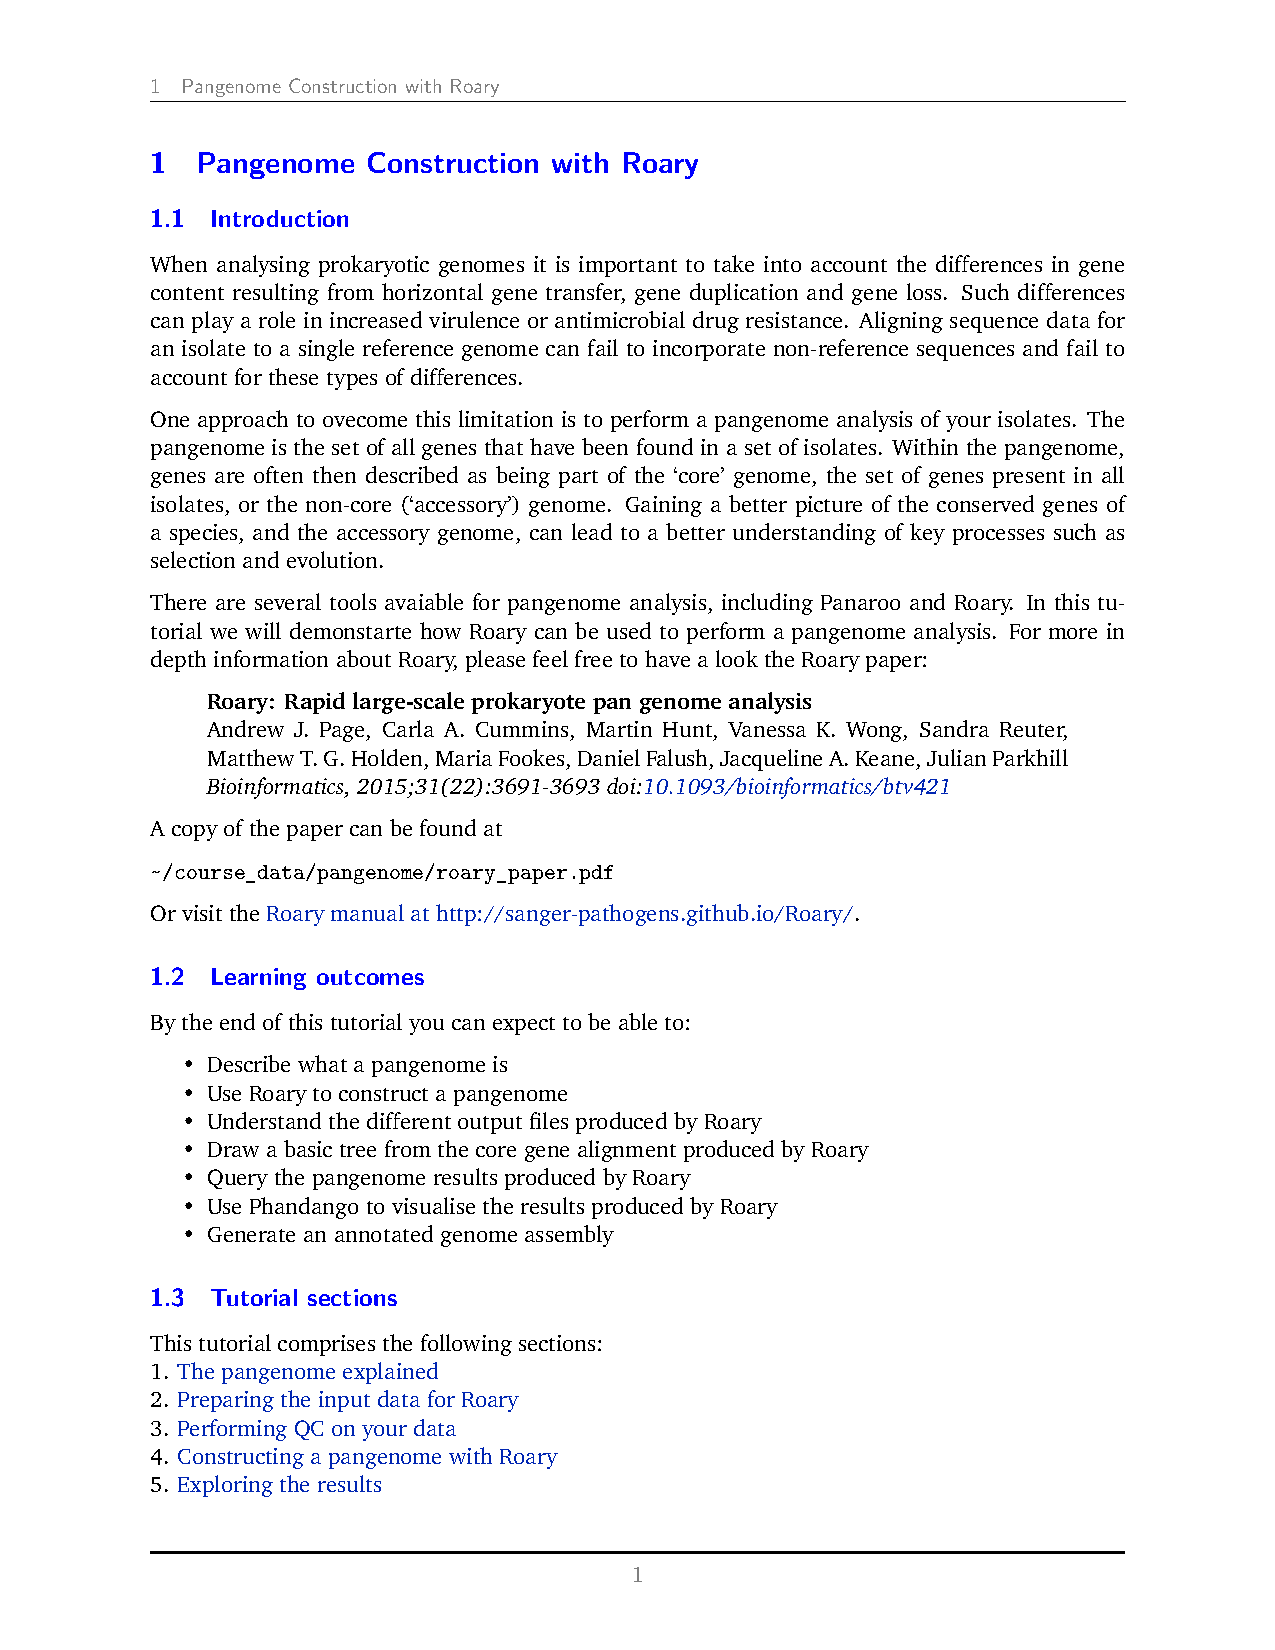
\includegraphics{img/pangenome.png}
\caption{Pan genome}
\end{figure}

    The pan, core and acessory genomes can provide important insight into
the genetic structure of prokaryotic genomes. By analysing the pangenome
we can gain a better understanding of key processes like evolution and
selection. Roay is a software tool that allows you to calculate the
pangenome for a set of isolates from a set of annotated genome
assemblies. It is fast and accurate and can conveniently be run on most
modern PCs. In this tutorial we are going to guide you through a
complete pangenome analysis, starting with annotation of the genome
assemblies, construction of the pangenome, and finally visualisation of
the results.

\hypertarget{check-your-understanding}{%
\subsection{Check your understanding}\label{check-your-understanding}}

\textbf{Q1: The pangenome contains:}\\
a) Only genes present in one isolate in a population\\
b) All genes from all isolates in a population\\
c) Only genes present in all isolates in a population

\textbf{Q2: Core genes are:}\\
a) Often important for basic cell functions\\
b) Present in only a subset of the isolates of a population\\
c) Often related to drug resistance

Now that you have an understanding of pangenomes, go to the next
session: \href{prepare_data.ipynb}{Preparing the input data for Roary}


    % Add a bibliography block to the postdoc



\newpage





    \hypertarget{preparing-the-input-data-for-roary}{%
\section{Preparing the input data for
Roary}\label{preparing-the-input-data-for-roary}}

\texttt{Roary} requires annotated genome assemblies in GFF3 format as
input.

A \textbf{genome assembly} is an attempted reconstruction of the
complete DNA sequence of an organism's genome from the short DNA
fragments generated by high-throughput sequencing technologies.

An \textbf{annotated genome assembly} is a genome assembly that has been
further analyzed to identify the various functional elements present in
the DNA sequence. It contains information about genes, regulatory
elements, non-coding regions, repetitive elements, and other
biologically relevant features.

For this tutorial, we have pre-prepared the genome assemblies of three
\textit{Streptococcus pneumoniae} isolates using sequence data obtained
from one of the public sequence archives, the ENA (European Nucleotide
Archives). The three assembled \textit{S. pneumoniae} genomes are located
in a directory called ``assemblies''.

    \begin{tcolorbox}[breakable, size=fbox, boxrule=1pt, pad at break*=1mm,colback=cellbackground, colframe=cellborder]
\prompt{In}{incolor}{ }{\boxspacing}
\begin{Verbatim}[commandchars=\\\{\}]
ls\PY{+w}{ }assemblies
\end{Verbatim}
\end{tcolorbox}

    These data and assemblies are also available for download from the ENA
and the accession numbers for the assemblies and the sequence data are
included below for reference.

\begin{longtable}[]{@{}lll@{}}
\toprule
Name & Genome Accession & Data Accession \\
\midrule
\endhead
sample1 & GCA\_900194945.1 & ERR657006 \\
sample2 & GCA\_900194155.1 & ERR657305 \\
sample3 & GCA\_900194195.1 & ERR657310 \\
\bottomrule
\end{longtable}

\hypertarget{annotating-genome-assemblies}{%
\subsection{Annotating genome
assemblies}\label{annotating-genome-assemblies}}

We must now annotate our genome assemblies to produce GFF3 files for
\texttt{Roary}. The GFF3 files must include the nucleotide sequence at
the end of the file, and to make it easier to identify which isolate
each gene came from, each GFF3 file should have a unique locus tag
(identifier) for the genes. \texttt{Prokka} is a tool that performs
genome annotation. All GFF3 files created by \texttt{Prokka} are valid
with \texttt{Roary} and therefore this is the recommended way of
generating the input files.

    To run \texttt{Prokka} on a single file using the default settings, you
would use something like:

\begin{verbatim}
prokka sample1.fasta
\end{verbatim}

If you have many assemblies, running this for each sample will soon
become tedious. Instead, we will use a for-loop to run \texttt{Prokka}
on all the fasta files in the assemblies directory.

    \begin{tcolorbox}[breakable, size=fbox, boxrule=1pt, pad at break*=1mm,colback=cellbackground, colframe=cellborder]
\prompt{In}{incolor}{ }{\boxspacing}
\begin{Verbatim}[commandchars=\\\{\}]
\PY{k}{for}\PY{+w}{ }F\PY{+w}{ }\PY{k}{in}\PY{+w}{ }assemblies/*.fasta\PY{p}{;}\PY{+w}{ }\PY{k}{do}\PY{+w}{ }
\PY{+w}{    }\PY{n+nv}{FILE}\PY{o}{=}\PY{l+s+si}{\PYZdl{}\PYZob{}}\PY{n+nv}{F}\PY{p}{\PYZsh{}\PYZsh{}*/}\PY{l+s+si}{\PYZcb{}}\PY{p}{;}\PY{+w}{ }\PY{n+nv}{PREFIX}\PY{o}{=}\PY{l+s+si}{\PYZdl{}\PYZob{}}\PY{n+nv}{FILE}\PY{p}{/.fasta/}\PY{l+s+si}{\PYZcb{}}\PY{p}{;}
\PY{+w}{    }prokka\PY{+w}{ }\PYZhy{}\PYZhy{}locustag\PY{+w}{ }\PY{n+nv}{\PYZdl{}PREFIX}\PY{+w}{ }\PYZhy{}\PYZhy{}outdir\PY{+w}{ }annotated\PYZus{}\PY{n+nv}{\PYZdl{}PREFIX}\PY{+w}{ }\PYZhy{}\PYZhy{}prefix\PY{+w}{ }\PY{n+nv}{\PYZdl{}PREFIX}\PY{+w}{ }\PY{n+nv}{\PYZdl{}F}\PY{p}{;}\PY{+w}{ }
\PY{k}{done}
\end{Verbatim}
\end{tcolorbox}

    For each fasta file in the assemblies directory, this will set FILE to
be the filename without the text `assemblies/' (e.g.~sample1.fasta ) and
set the value of PREFIX to be the text found before `.fasta'
(e.g.~sample1) and the value of \$F will be the path to the fasta file
(assemblies/sample1.fasta). We have also used the following options for
Prokka:

\begin{longtable}[]{@{}ll@{}}
\toprule
Option & Description \\
\midrule
\endhead
\texttt{-\/-locustag} & The locus tag prefix \\
\texttt{-\/-outdir} & The directory to put the output \\
\texttt{-\/-prefix} & The prefix for the output files \\
\bottomrule
\end{longtable}

By providing a unique value for the \texttt{-\/-locustag} option we make
it easier to identify which sample different genes came from when we
look at the results from Roary. The \texttt{-\/-outdir} and
\texttt{-\/-prefix} options will make it easier for us to keep track of
our files.

This is going to take around 5 minutes or longer to run, so be patient.
Perhaps read the next section \href{qc.ipynb}{Performing QC on your
data} come back here when Prokka is finished running.

Once this has finished, you should have three new directories called
\texttt{annotated\_sample1}, \texttt{annotated\_sample2} and
\texttt{annotated\_sample3}. Have a look to see that it worked:

    \begin{tcolorbox}[breakable, size=fbox, boxrule=1pt, pad at break*=1mm,colback=cellbackground, colframe=cellborder]
\prompt{In}{incolor}{ }{\boxspacing}
\begin{Verbatim}[commandchars=\\\{\}]
ls\PY{+w}{ }\PYZhy{}l
\end{Verbatim}
\end{tcolorbox}

    \begin{tcolorbox}[breakable, size=fbox, boxrule=1pt, pad at break*=1mm,colback=cellbackground, colframe=cellborder]
\prompt{In}{incolor}{ }{\boxspacing}
\begin{Verbatim}[commandchars=\\\{\}]
ls\PY{+w}{ }\PYZhy{}l\PY{+w}{ }annotated\PYZus{}sample1
\end{Verbatim}
\end{tcolorbox}

    As you can see, for sample1 we now have a number of annotation files.
There is more information about the different output files, along with
information about other usage options, on the
\href{https://github.com/tseemann/prokka}{Prokka GitHub page
(https://github.com/tseemann/prokka)}. For now, we are only interrested
in the GFF files that were generated as this is what we are going to use
as input for Roary.

\hypertarget{check-your-understanding}{%
\subsection{Check your understanding}\label{check-your-understanding}}

\textbf{Q3: Why do we need to run Prokka?}\\
a) It will perform QC on our data\\
b) It will annotate our data\\
c) We don't, Roary can handle fasta files as input

\textbf{Q4: Why do we use the --locustag option when we run Prokka?}\\
a) To make it easier to keep track of the output files\\
b) Because Roary won't work without it\\
c) To make the Roary results easier to interpret

Now continue to the next section of the tutorial:
\href{qc.ipynb}{Performing QC on your data}.


    % Add a bibliography block to the postdoc



\newpage





    \hypertarget{performing-qc-on-your-data}{%
\section{Performing QC on your data}\label{performing-qc-on-your-data}}

The results you can get from any analysis will only ever be as good as
the data you put into it. To avoid spending countless hours performing
analysis without receiving any satisfactory results, or worse yet
erroneous or misleading results, it is important to QC your data before
starting. There are a number of checks you can make to ensure you are
dealing with good quality data, and we will walk you through some of
them here.

\hypertarget{contamination}{%
\subsection{Contamination}\label{contamination}}

In order to get meaningful results from \texttt{Roary}, the samples
should be closely related. If you have lots of contamination in your
data, for instance if one of your samples is from a different species,
you will get very few genes in your core genome, if any at all.

It is always a good idea to check that your samples are the species you
expect them to be. You can use tools such as \texttt{Bactinspector} or
\href{https://www.ebi.ac.uk/research/enright/software/kraken}{\texttt{Kraken}
(https://www.ebi.ac.uk/research/enright/software/kraken)} for this.
\texttt{Roary} has a qc option that will run \texttt{Kraken} for you and
generate a report listing the top species of all the samples.

We will not run \texttt{Kraken} now but an example report may look
something like this:

    \begin{figure}
\centering
\includegraphics{img/qc_report.png}
\caption{QC report}
\end{figure}

    As we expected, these three samples are all of the same species. Let's
assume that we had an additional fourth sample and we run \texttt{Roary}
with the qc option, we get the following output:

    \begin{figure}
\centering
\includegraphics{img/qc_contamination.png}
\caption{QC report with contamination}
\end{figure}

    This tells us that the most prevalent species in sample 4 is in fact
\textit{Escherichia coli} so we will exclude this sample from our analysis
before we carry on.

\hypertarget{coverage}{%
\subsection{Coverage}\label{coverage}}

To get reasonable quality assemblies, you need a genome coverage of at
least 30x. Remember to get a quick estimate of your coverage, you can
divide the number of bases in your sequence data with the number of
bases in the reference genome of the species. For the samples used in
this tutorial, the coverage is listed below. The genome of \textit{S.
pneumoniae} is approximately 2,200,000 bases.

\begin{longtable}[]{@{}lll@{}}
\toprule
Sample & No.~of Bases & Coverage \\
\midrule
\endhead
sample1 & 262705400 & 120x \\
sample2 & 218026200 & 99x \\
sample3 & 173524000 & 79x \\
\bottomrule
\end{longtable}

\hypertarget{assembly-size}{%
\subsection{Assembly size}\label{assembly-size}}

The size of the assemblies can also provide a useful hint. If one of the
assemblies is much smaller or bigger than the others there is a chance
that this is not of the same species as the rest.

\hypertarget{fragmented-assemblies}{%
\subsection{Fragmented assemblies}\label{fragmented-assemblies}}

If the assemblies are very fragmented (thousands of contigs), the genes
may be too fragmented for inferring the pangenome.

These are just some of the most basic things that you can do to make
sure your data looks ok. There is much more that can be done but we
won't go into any further detail in this tutorial.

To generate some basic metrics about genome assemblies you can use the
\texttt{assembly-stats} tools.

    \begin{tcolorbox}[breakable, size=fbox, boxrule=1pt, pad at break*=1mm,colback=cellbackground, colframe=cellborder]
\prompt{In}{incolor}{ }{\boxspacing}
\begin{Verbatim}[commandchars=\\\{\}]
assembly\PYZhy{}stats\PY{+w}{ }assemblies/sample1.fasta
\end{Verbatim}
\end{tcolorbox}

    \hypertarget{check-your-understanding}{%
\subsection{Check your understanding}\label{check-your-understanding}}

\textbf{Q5: Why is it important to QC your data?}

\textbf{Q6: You're not getting any core genes when you run Roary. What
could be the reason?}

\textbf{Q7: What is the size of the assembly for sample1?}

\textbf{Q8: How many contigs are in the assembly of sample1?}

    Now you should be ready to run Roary to construct a pangenome, so go to
the next section, \href{run_roary.ipynb}{Constructing a Pangenome using
Roary}.


    % Add a bibliography block to the postdoc



\newpage





    \hypertarget{constructing-a-pangenome-with-roary}{%
\section{Constructing a Pangenome with
Roary}\label{constructing-a-pangenome-with-roary}}

At this stage you should have three GFF files generated by
\texttt{Prokka}, each in its own directory. Provided your QC looked ok,
you are now ready to run \texttt{Roary} to generate the pangenome.

We are going to run \texttt{Roary} twice, first with the default
settings, and then using \texttt{MAFFT} to generate a core gene
alignment. For both of these runs we will want all the annotation files
in the same directory, so lets take a copy of them to our current
directory:

    \begin{tcolorbox}[breakable, size=fbox, boxrule=1pt, pad at break*=1mm,colback=cellbackground, colframe=cellborder]
\prompt{In}{incolor}{ }{\boxspacing}
\begin{Verbatim}[commandchars=\\\{\}]
cp\PY{+w}{ }annotated\PYZus{}sample*/*.gff\PY{+w}{ }.
\end{Verbatim}
\end{tcolorbox}

    \hypertarget{run-roary-with-default-settings}{%
\subsection{Run Roary with default
settings}\label{run-roary-with-default-settings}}

To run \texttt{Roary} with the default settings all you need to do is
run \texttt{roary\ *.gff} and it will create a pangenome using all GFF
files in the current directory. Try the following command:

    \begin{tcolorbox}[breakable, size=fbox, boxrule=1pt, pad at break*=1mm,colback=cellbackground, colframe=cellborder]
\prompt{In}{incolor}{ }{\boxspacing}
\begin{Verbatim}[commandchars=\\\{\}]
roary\PY{+w}{ }\PYZhy{}f\PY{+w}{ }output\PYZus{}no\PYZus{}alignment\PY{+w}{ }*.gff
\end{Verbatim}
\end{tcolorbox}

    We want to run Roary twice with different settings, so in order to keep
track of our output files from each run we will use the \textbf{-f}
option to specify the name of the ouptut directory where \texttt{Roary}
should put the results. This will run for a few minutes.

We will have a closer look at the results in the next section, so for
now let us just see that there are some output files in the directroy we
asked \texttt{Roary} to create:

    \begin{tcolorbox}[breakable, size=fbox, boxrule=1pt, pad at break*=1mm,colback=cellbackground, colframe=cellborder]
\prompt{In}{incolor}{ }{\boxspacing}
\begin{Verbatim}[commandchars=\\\{\}]
ls\PY{+w}{ }\PYZhy{}l\PY{+w}{ }output\PYZus{}no\PYZus{}alignment
\end{Verbatim}
\end{tcolorbox}

    \hypertarget{run-roary-with-mafft}{%
\subsection{Run Roary with MAFFT}\label{run-roary-with-mafft}}

But we want to generate a multi-FASTA alignment of the core genes so
that we can draw a phylogenetic tree. So try:

    \begin{tcolorbox}[breakable, size=fbox, boxrule=1pt, pad at break*=1mm,colback=cellbackground, colframe=cellborder]
\prompt{In}{incolor}{ }{\boxspacing}
\begin{Verbatim}[commandchars=\\\{\}]
roary\PY{+w}{ }\PYZhy{}f\PY{+w}{ }output\PYZus{}with\PYZus{}alignment\PY{+w}{ }\PYZhy{}e\PY{+w}{ }\PYZhy{}\PYZhy{}mafft\PY{+w}{ }\PYZhy{}p\PY{+w}{ }\PY{l+m}{2}\PY{+w}{ }*.gff
\end{Verbatim}
\end{tcolorbox}

    Here we have run \texttt{Roary} again, but this time with some more
options.

\begin{longtable}[]{@{}ll@{}}
\toprule
Option & Description \\
\midrule
\endhead
\texttt{-e} & Create a multi-FASTA alignment of the core genes \\
\texttt{-\/-mafft} & Use with -e to use MAFFT instead of PRANK \\
\texttt{-p} & Number of threads to use \\
\bottomrule
\end{longtable}

By default, \texttt{Roary} will use \texttt{PRANK} when the \texttt{-e}
option is speified. It is accurate but slow. \texttt{MAFFT} is less
accurate but very fast so we are going to use this instead by specifying
the \texttt{-\/-mafft} option. To further speed things up, we are going
to use 2 threads (the \texttt{-p} option). For all usage options, you
can have a look at the
\href{https://sanger-pathogens.github.io/Roary/}{Roary website
(https://sanger-pathogens.github.io/Roary/)}.

    This will take a bit longer to run than the previous command, maybe 5 or
10 minutes, perhaps answer the questions at the end of this section
while waiting for this to complete.

Once finished you should have a directory called
\texttt{output\_with\_alignment} containing the output files, this time
including a core\_gene\_alignment.aln file. Just quickly check that this
is the case.

    \begin{tcolorbox}[breakable, size=fbox, boxrule=1pt, pad at break*=1mm,colback=cellbackground, colframe=cellborder]
\prompt{In}{incolor}{ }{\boxspacing}
\begin{Verbatim}[commandchars=\\\{\}]
ls\PY{+w}{ }\PYZhy{}l\PY{+w}{ }output\PYZus{}with\PYZus{}alignment
\end{Verbatim}
\end{tcolorbox}

    \hypertarget{check-your-understanding}{%
\subsection{Check your understanding}\label{check-your-understanding}}

\textbf{Q9: Why do we want to run Roary with MAFFT?}\\
a) Because it's quicker than to run Roary without the -e option\\
b) To get more accurate results\\
c) To generate a core gene alignment

\textbf{Q10: Why do we use the -p otion?}\\
a) We have to when we use MAFFT\\
b) To speed up the run\\
c) To get a nice tree

Now go to the next section: \href{results.ipynb}{Exploring the results}.


    % Add a bibliography block to the postdoc



\newpage





    \hypertarget{exploring-the-results}{%
\section{Exploring the results}\label{exploring-the-results}}

\hypertarget{output-files}{%
\subsection{Output files}\label{output-files}}

Let's have a look at the results. We will focus on the output from the
second run as this will be the same as the first run but will also
include the core gene alignment produced by \texttt{MAFFT}. We will
start by looking at the most important output files and after this we
will look at how you can query your pangenome and draw a basic tree form
the core gene alignment.

    \begin{tcolorbox}[breakable, size=fbox, boxrule=1pt, pad at break*=1mm,colback=cellbackground, colframe=cellborder]
\prompt{In}{incolor}{ }{\boxspacing}
\begin{Verbatim}[commandchars=\\\{\}]
ls\PY{+w}{ }output\PYZus{}with\PYZus{}alignment
\end{Verbatim}
\end{tcolorbox}

    \hypertarget{summary_statistics.txt}{%
\subsubsection{summary\_statistics.txt}\label{summary_statistics.txt}}

The summary\_statistics.txt file contains a summary of the number of
genes in the pan, core and accessory genomes. It provides an overview of
the genes and how frequently they occur in the input isolates. Usually,
you can expect the total number of genes in this file to be about 1,000
genes per million bases of your species reference genome. In this case,
the genomes are around 2 million bases, so we would expect a total
number of genes to be in the order of 2,000. Let's have a look and see
if this is the case.

    \begin{tcolorbox}[breakable, size=fbox, boxrule=1pt, pad at break*=1mm,colback=cellbackground, colframe=cellborder]
\prompt{In}{incolor}{ }{\boxspacing}
\begin{Verbatim}[commandchars=\\\{\}]
cat\PY{+w}{ }output\PYZus{}with\PYZus{}alignment/summary\PYZus{}statistics.txt
\end{Verbatim}
\end{tcolorbox}

    As you can see, we have around 2,500 genes which seems about right. If
you get a lot fewer or many more genes than expected this could be an
indication of an issue with your input data, for example contamination.

\hypertarget{gene_presence_absence}{%
\subsubsection{gene\_presence\_absence}\label{gene_presence_absence}}

The gene\_presence\_absence files lists each gene and which samples it
is present in. The .csv file can be opened in Excel.

Let's have a look at the first ten lines of the file:

    \begin{tcolorbox}[breakable, size=fbox, boxrule=1pt, pad at break*=1mm,colback=cellbackground, colframe=cellborder]
\prompt{In}{incolor}{ }{\boxspacing}
\begin{Verbatim}[commandchars=\\\{\}]
head\PY{+w}{ }output\PYZus{}with\PYZus{}alignment/gene\PYZus{}presence\PYZus{}absence.csv
\end{Verbatim}
\end{tcolorbox}

    The columns are tab separated and contains the following information:

\begin{enumerate}
\def\labelenumi{\arabic{enumi}.}
\tightlist
\item
  The gene name (the most frequently occurring gene name from the
  sequences in the cluster)
\item
  A non unique gene name
\item
  Functional annotation (the most frequently occurring functional
  annotation from the cluster)
\item
  Number of isolates in the cluster
\item
  Number of sequences in the cluster
\item
  Average number of sequences per isolate (normally 1)
\item
  Genome fragment
\item
  Order within fragment
\item
  Accessory fragment
\item
  Accessory order within fragment
\item
  Comments on the quality of the cluster
\item
  Minimum sequence length in nucleotides of the cluster
\item
  Maximum sequence length in nucleotides of the cluster
\item
  Average sequence length in nucleotides of the cluster
\item
  Presence and absence of genes in each sample, with the corresponding
  source Gene ID
\end{enumerate}

The .Rtab file contains a tab delimited binary matrix with the precence
and abscence of each gene in each sample. This makes it easy to load
into R using the read.table function, giving you access to a number of
useful tools. The first row is the header containing the name of each
sample, and the first column contains the gene name. In the matrix, 1
indicates the gene is present in the sample and 0 indicates it is
absent.

\hypertarget{pan_genome_reference.fa}{%
\subsubsection{pan\_genome\_reference.fa}\label{pan_genome_reference.fa}}

This fasta file contains a single nucleotide sequence from each of the
clusters in the pan genome. The name of each sequence is the source
sequence ID followed by the cluster it came from.

\hypertarget{rtab}{%
\subsubsection{.Rtab}\label{rtab}}

Roary comes packaged with a script called create\_pan\_genome\_plots.R.
It requires R and the R-package ggplot2, and can be used to generate
graphs from the .Rtab files, showing how the pan genome varies as
genomes are added.

\hypertarget{accessory_binary_genes.fa.newick}{%
\subsubsection{accessory\_binary\_genes.fa.newick}\label{accessory_binary_genes.fa.newick}}

This is a tree in newick format, created using the binary presence and
absence of accessory genes. It can for example be viewed in
\href{http://tree.bio.ed.ac.uk/software/figtree/}{FigTree}. The tree is
only a tough estmate, generated to provide a basic overview of the data.
To generate a more accurate tree, we will use the core gene alignment a
bit further on.

\hypertarget{core_gene_alignment.aln}{%
\subsubsection{core\_gene\_alignment.aln}\label{core_gene_alignment.aln}}

This is the multi-FASTA alignment of core genes that we created in the
second run, using MAFFT. We will soon use this as input to build a
phylogenetic tree.

\hypertarget{clustered_proteins}{%
\subsubsection{clustered\_proteins}\label{clustered_proteins}}

In this file each line lists the sequences in a cluster. We will use
this later on in the tutorial to query the pan genome.

    For more information about the different output files, including some
that we haven't mentioned here, please feel free to have a look at the
\href{https://sanger-pathogens.github.io/Roary/}{Roary web page}.

    \hypertarget{query-the-pan-genome}{%
\subsection{Query the pan genome}\label{query-the-pan-genome}}

Roary comes with a script called query\_pan\_genome that can be used to
examine the gene differences between groups of isolates. To have a look
at the usage options for this script, you can do:

\begin{verbatim}
query_pan_genome -h
\end{verbatim}

This will show you the following usage options:

\begin{verbatim}
Usage: query_pan_genome [options] *.gff
Perform set operations on the pan genome to see the gene differences
between groups of isolates.

Options: -g STR    groups filename [clustered_proteins]
         -a STR    action (union/intersection/complement/gene_multifasta/
                     difference) [union]
         -c FLOAT  percentage of isolates a gene must be in to be core [99]
         -o STR    output filename [pan_genome_results]
         -n STR    comma separated list of gene names for use with
                     gene_multifasta action
         -i STR    comma separated list of filenames, comparison set one
         -t STR    comma separated list of filenames, comparison set two
         -v        verbose output to STDOUT
         -h        this help message

Examples:
Union of genes found in isolates
         query_pan_genome -a union *.gff

Intersection of genes found in isolates (core genes)
         query_pan_genome -a intersection *.gff

Complement of genes found in isolates (accessory genes)
         query_pan_genome -a complement *.gff

Extract the sequence of each gene listed and create multi-FASTA files
         query_pan_genome -a gene_multifasta -n gryA,mecA,abc *.gff

Gene differences between sets of isolates
         query_pan_genome -a difference --input_set_one 1.gff,2.gff --input_set_two 3.gff,4.gff,5.gff

For further info see: http://sanger-pathogens.github.io/Roary/
\end{verbatim}

    As you can see, this also shows us some example uses. Try the first
example:

    \begin{tcolorbox}[breakable, size=fbox, boxrule=1pt, pad at break*=1mm,colback=cellbackground, colframe=cellborder]
\prompt{In}{incolor}{ }{\boxspacing}
\begin{Verbatim}[commandchars=\\\{\}]
query\PYZus{}pan\PYZus{}genome\PY{+w}{ }\PYZhy{}a\PY{+w}{ }union\PY{+w}{ }\PYZhy{}g\PY{+w}{ }output\PYZus{}with\PYZus{}alignment/clustered\PYZus{}proteins\PY{+w}{ }*.gff
\end{Verbatim}
\end{tcolorbox}

    This will give us a file called pan\_genome\_results that contains a
list of all genes in all samples, i.e.~the pangenome. Have a look at the
first ten lines of the newly generated file:

    \begin{tcolorbox}[breakable, size=fbox, boxrule=1pt, pad at break*=1mm,colback=cellbackground, colframe=cellborder]
\prompt{In}{incolor}{ }{\boxspacing}
\begin{Verbatim}[commandchars=\\\{\}]
head\PY{+w}{ }pan\PYZus{}genome\PYZus{}results
\end{Verbatim}
\end{tcolorbox}

    The list contains the names of the gene clusters (this is usually the
most frequently occurring gene name from the sequences in the cluster
or, if there is no gene name, a generic unique name group\_XXX). For
each cluster, there is a tab separated list of each sample specific gene
belonging in that cluster.

In a similar way, you can use query\_pan\_genome to get a list of the
core genes:

\begin{verbatim}
query_pan_genome -a intersection \
    -g output_with_alignment/clustered_proteins *.gff
\end{verbatim}

and a list of the accessory genes:

\begin{verbatim}
query_pan_genome -a complement \
    -g output_with_alignment/clustered_proteins *.gff
\end{verbatim}

You can also use query\_pan\_genome to extract the protein sequences for
genes you are particularly interested in.

    \begin{tcolorbox}[breakable, size=fbox, boxrule=1pt, pad at break*=1mm,colback=cellbackground, colframe=cellborder]
\prompt{In}{incolor}{ }{\boxspacing}
\begin{Verbatim}[commandchars=\\\{\}]
query\PYZus{}pan\PYZus{}genome\PY{+w}{ }\PYZhy{}a\PY{+w}{ }gene\PYZus{}multifasta\PY{+w}{ }\PYZhy{}g\PY{+w}{ }output\PYZus{}with\PYZus{}alignment/clustered\PYZus{}proteins\PY{+w}{ }\PYZhy{}n\PY{+w}{ }patB,mnmG,hsdM\PY{+w}{ }*.gff
\end{Verbatim}
\end{tcolorbox}

    Note this command is shown here split over multiple lines. It should be
typed as one command in one line in the terminal window.

The \textbf{-a} option species the action (create a multi-FASTA file of
protein sequences) and the \textbf{-n} option specifies a comma
separated list of the cluster names (patB,mnmG,hsdM).

You should have three new files, one for each gene you specified.

    \begin{tcolorbox}[breakable, size=fbox, boxrule=1pt, pad at break*=1mm,colback=cellbackground, colframe=cellborder]
\prompt{In}{incolor}{ }{\boxspacing}
\begin{Verbatim}[commandchars=\\\{\}]
ls\PY{+w}{ }*.fa
\end{Verbatim}
\end{tcolorbox}

    \begin{tcolorbox}[breakable, size=fbox, boxrule=1pt, pad at break*=1mm,colback=cellbackground, colframe=cellborder]
\prompt{In}{incolor}{ }{\boxspacing}
\begin{Verbatim}[commandchars=\\\{\}]
Have\PY{+w}{ }a\PY{+w}{ }look\PY{+w}{ }at\PY{+w}{ }the\PY{+w}{ }\PY{l+s+sb}{`}pan\PYZus{}genome\PYZus{}results\PYZus{}patB.fa\PY{l+s+sb}{`}\PY{+w}{ }file:
\end{Verbatim}
\end{tcolorbox}

    \begin{tcolorbox}[breakable, size=fbox, boxrule=1pt, pad at break*=1mm,colback=cellbackground, colframe=cellborder]
\prompt{In}{incolor}{ }{\boxspacing}
\begin{Verbatim}[commandchars=\\\{\}]
cat\PY{+w}{ }pan\PYZus{}genome\PYZus{}results\PYZus{}patB.fa
\end{Verbatim}
\end{tcolorbox}

    This multi-FASTA file contains the three protein sequences in the
specified cluster (patB).

There is yet more functionality of query\_pan\_genome, but we won't go
into that here. For further information, please feel free to visit the
\href{https://sanger-pathogens.github.io/Roary/}{Roary web page
(https://sanger-pathogens.github.io/Roary/)}.

    \hypertarget{draw-a-tree-form-the-core-gene-alignment}{%
\subsection{Draw a tree form the core gene
alignment}\label{draw-a-tree-form-the-core-gene-alignment}}

The tree created by \texttt{Roary} (accessory\_binary\_genes.fa.newick)
is just a quick tree to provide a rough insight into the data. To create
a more accurate tree you can use the core gene alignment as input to a
tree building software of your choice.
\href{https://sco.h-its.org/exelixis/web/software/raxml/index.html}{RAxML
(https://sco.h-its.org/exelixis/web/software/raxml/index.html)} is very
accurate, however it is also fairly slow so in this tutorial we are
going to use \href{http://www.microbesonline.org/fasttree/}{FastTree
(http://www.microbesonline.org/fasttree/)}.

To create a tree in Newick format
({[}https://evolution.genetics.washington.edu/phylip/newicktree.html{]})(https://evolution.genetics.washington.edu/phylip/newicktree.html)
from a nucleotide alignment using a generalized time-reversible model
(the -gtr option), do:

    \begin{tcolorbox}[breakable, size=fbox, boxrule=1pt, pad at break*=1mm,colback=cellbackground, colframe=cellborder]
\prompt{In}{incolor}{ }{\boxspacing}
\begin{Verbatim}[commandchars=\\\{\}]
fasttree\PY{+w}{ }\PYZhy{}nt\PY{+w}{ }\PYZhy{}gtr\PY{+w}{ }output\PYZus{}with\PYZus{}alignment/core\PYZus{}gene\PYZus{}alignment.aln\PY{+w}{ }\PYZgt{}\PY{+w}{ }tree.newick
\end{Verbatim}
\end{tcolorbox}

    The tree in this case will look like:

\begin{verbatim}
(sample1:0.006228253,sample2:0.002364375,sample3:0.002920483);
\end{verbatim}

We can view this in \texttt{iTOl} or \texttt{FigTree}, which will look
something like:


\begin{center}
\includegraphics[Phylogenetic tree]{img/my_tree.newick.png}
\end{center}


In the event that you did not run this step, a copy of tree.newick has
been placed in the \texttt{tree} directory for the next section of this
tutorial.

\hypertarget{check-your-understanding}{%
\subsection{Check your understanding}\label{check-your-understanding}}

\textbf{Q11: Approximately how many genes would you expect to see in the
summary\_statistics.txt file if you are working with a species with a
genome size of 5,000,000 bases?}\\
a) 500\\
b) 5000\\
c) 50,000

\textbf{Q12: What does the accessory\_binary\_genes.fa.newick file
provide?}\\
a) A pylogenetic tree ready for publishing\\
b) Nothing, it is useless\\
c) A quick insight to the data

\textbf{Q13: For query\_pan\_genome, what option should you use to get
the accessory genome?}\\
a) union\\
b) intersection\\
c) complement

Now that you are familiar with the output files produced by Roary, let's
make use of them by \href{phandango.ipynb}{visualising the results using
Phandango}.


    % Add a bibliography block to the postdoc



\newpage





    \hypertarget{visualising-the-results-with-phandango}{%
\section{Visualising the results with
phandango}\label{visualising-the-results-with-phandango}}

\href{http://phandango.net/}{\texttt{Phandango} (http://phandango.net/)}
is a web based tool for visualising genomic analysis results such as
phylogenetic trees and the output of \texttt{Roary} and other tools.
Using phandango is straightforward, you just drag your files onto the
browser and drop them and \texttt{Phandango} will display them for you
automatically. For more in depth information please feel free to have a
look around the
\href{https://github.com/jameshadfield/phandango/wiki}{phandango wiki
page (https://github.com/jameshadfield/phandango/wiki)}.

In this section of the tutorial we are going to use \texttt{Phandango}
to look at the pylogenetic tree we generated using \texttt{FastTree},
and the gene\_presence\_absence.csv file we obtained from
\texttt{Roary}. Simply dragging the two files and droping them on the
phandango front page will give you the following view:


\begin{center}
\includegraphics[phandango]{img/phandango.png}
\end{center}


    The image shows our tree compared to a matrix with the presence and
absence of genes in the pan genome. The graph on the bottom right
provides a summary of the matrix above, indicating the percentage of
isolates carrying a gene at each position.

You can zoom in on a particular area you are interested in simply by
scrolling, and to see the annotation for a particular gene you can place
your pointer over the corresponding bar at the top of the page, like in
the figure below.


\begin{center}
\includegraphics[zoom]{img/phandango_zoom.png}
\end{center}


In this case we are looking at a gene called \textit{moeB}. We can see
that the gene is present in sample2 and sample3, but not in sample1, and
that the product is an Molybdopterin-synthase adenylyltransferase.

Go ahead and experiment with \texttt{Phandango}. You can alter the
layout in \textit{settings} in the navigation bar at the top of the page,
or by clicking and dragging the grey circles on the page. To download
the current view in svg format, simply press \textit{p}.

\hypertarget{check-your-understanding}{%
\subsection{Check your understanding}\label{check-your-understanding}}

\textbf{In Phandango, zoom in on the gene cluster at position 25080.}

\textbf{Q14: What is the name of this gene cluster?}

\textbf{Q15: Is this a core gene?}

This tutorial has shown you how to construct a pangenome for a set of
genome assemblies. The final section of this turorial will discuss how
to generate genome assemblies from short read sequence data. OK, let's
\href{assembly.ipynb}{generate some genome assemblies}!


    % Add a bibliography block to the postdoc



\newpage





    \hypertarget{creating-genome-assemblies}{%
\section{Creating genome assemblies}\label{creating-genome-assemblies}}

Genome assembly is the process of taking a large number of fragments of
DNA and putting them back together to create a representation of the
original DNA sequence from which they originated.

    \begin{figure}
\centering
\includegraphics{img/genome_assembly.png}
\caption{Genome assembly}
\end{figure}

    Many genomes contain large numbers of repeat sequences. Often these
repeats are thousands of nucleotides long, and some occur in many
different locations in the genome. This makes genome assembly a very
difficult computational problem to solve. However, there are many genome
assembly tools that exist that can produce long contiguous sequences
(contigs) from sequencing reads. The assembly tool that you use will be
determined by different factors, largely this will be the length of the
sequencing reads and the sequencing technology used to produce the
reads.

    First, check you are in the correct directory.

    \begin{tcolorbox}[breakable, size=fbox, boxrule=1pt, pad at break*=1mm,colback=cellbackground, colframe=cellborder]
\prompt{In}{incolor}{ }{\boxspacing}
\begin{Verbatim}[commandchars=\\\{\}]
\PY{n+nb}{pwd}
\end{Verbatim}
\end{tcolorbox}

    It should display something like:

\texttt{/home/manager/course\_data/pangenome/data}

    \hypertarget{assemble-a-genome-with-spades}{%
\subsection{Assemble a genome with
SPAdes}\label{assemble-a-genome-with-spades}}

Now we are going to use the \texttt{SPAdes} assembly tool to generate an
assembly. As always it is a good idea to get a look at the options that
a program accepts using the -h option. SPAdes is actually written in
python and the base script name is ``spades.py''.

    \begin{tcolorbox}[breakable, size=fbox, boxrule=1pt, pad at break*=1mm,colback=cellbackground, colframe=cellborder]
\prompt{In}{incolor}{ }{\boxspacing}
\begin{Verbatim}[commandchars=\\\{\}]
spades.py\PY{+w}{ }\PYZhy{}h
\end{Verbatim}
\end{tcolorbox}

    To assemble the data for sample ERR657310 using \texttt{SPAdes} and
default parameters use:

    \begin{tcolorbox}[breakable, size=fbox, boxrule=1pt, pad at break*=1mm,colback=cellbackground, colframe=cellborder]
\prompt{In}{incolor}{ }{\boxspacing}
\begin{Verbatim}[commandchars=\\\{\}]
spades.py\PY{+w}{ }\PYZhy{}\PYZhy{}pe1\PYZhy{}1\PY{+w}{ }fastq/ERR657310\PYZus{}1.fastq.gz\PY{+w}{ }\PYZhy{}\PYZhy{}pe1\PYZhy{}2\PY{+w}{ }fastq/ERR657310\PYZus{}2.fastq.gz\PY{+w}{ }\PYZhy{}\PYZhy{}only\PYZhy{}assembler\PY{+w}{ }\PYZhy{}\PYZhy{}careful\PY{+w}{ }\PYZhy{}o\PY{+w}{ }ERR657310\PY{+w}{ }\PYZhy{}k\PY{+w}{ }\PY{l+m}{33},43,53,63\PY{+w}{ }\PYZhy{}\PYZhy{}threads\PY{+w}{ }\PY{l+m}{2}
\end{Verbatim}
\end{tcolorbox}

    Note this command is split over multiple lines but should be typed as
one command in one line in the terminal window. This may take some time
to run so please be patient.

\texttt{SPAdes} (St.~Petersburg genome assembler) is a genome assembly
algorithm which was designed for single cell and multi-cell bacterial
data sets. Therefore, it might not be suitable for large genomes
projects. \texttt{SPAdes} works with Ion Torrent, PacBio, Oxford
Nanopore, and Illumina paired-end, mate-pairs and single reads.

Here we are using it to assemble Illumina paired end data. Take a look
at the parameters passed to SPAdes, what do the different parameters
mean?

    When the assembly is complete look at the files that were produced by
SPAdes:

    \begin{tcolorbox}[breakable, size=fbox, boxrule=1pt, pad at break*=1mm,colback=cellbackground, colframe=cellborder]
\prompt{In}{incolor}{ }{\boxspacing}
\begin{Verbatim}[commandchars=\\\{\}]
ls\PY{+w}{ }ERR657310
\end{Verbatim}
\end{tcolorbox}

    As you can see from listing the contents of the output \texttt{sample3}
directory, several new files have been generated. There are two files
that I consider to be the most important. * \texttt{contigs.fasta} -
this is the actual result of all the different contigs that were
created. For circular chromosomes (such as plasmids) the goal would be
that there is a single contig meaning that all of the reads were able to
close the circle. * \texttt{spades.log} - this has the information about
the completed run that you can use to compare different samples or
conditions in the event that you are interested trying to optimize the
command options, as would likely be the case if you were trying to
assemble the best reference possible.

    \hypertarget{assembly-metrics}{%
\subsection{Assembly metrics}\label{assembly-metrics}}

To generate metrics to assess the quality of the assembly you can use a
program called \texttt{assembly-stats}. It displays the number of
contigs, the mean contig size and a lot of other useful metrics about
the assembly. These numbers can be used to assess the quality of your
assembly.

    \begin{tcolorbox}[breakable, size=fbox, boxrule=1pt, pad at break*=1mm,colback=cellbackground, colframe=cellborder]
\prompt{In}{incolor}{ }{\boxspacing}
\begin{Verbatim}[commandchars=\\\{\}]
assembly\PYZhy{}stats\PY{+w}{ }ERR657310/contigs.fasta
\end{Verbatim}
\end{tcolorbox}

    Now look at the output of \texttt{assembly-stats} and answer the
questions below

    \hypertarget{check-your-understanding}{%
\subsection{Check your understanding}\label{check-your-understanding}}

\textbf{Q16: What is the size of the assembly?}

\textbf{Q17: How many contigs did it assemble into?}

\textbf{Q18: What is the largest contig?}

\textbf{Q19: What is the N50?}

\textbf{Q20: Is this a good assembly?}

    Another good software tool to assess the quality of your assemblies is
\href{http://bioinf.spbau.ru/quast}{\texttt{Quast}
(http://bioinf.spbau.ru/quast)}. However, we do not have time here to
cover the use of Quast here.

    \hypertarget{genome-assembly-pipelines}{%
\subsection{Genome assembly pipelines}\label{genome-assembly-pipelines}}

Unfortunately, to generate high quality genome assemblies it is usually
not as straightforward as just running an assembly tool like
\texttt{SPAdes}. There are several pre-processing and post-processing
steps than need to be carried out in order to improve the chances of
creating a good quality assembly. These steps can include:

\begin{itemize}
\tightlist
\item
  Trimming reads to remove low quality bases
\item
  Trimming reads to remove sequence adapter
\item
  Correcting sequencing errors in the reads
\item
  Downsampling the data to allow the assembly to run within reasonable
  time and memory
\item
  Mapping reads back to the assembly to correct errors in the assembly
\item
  Filtering small/low quality contigs from the assembly
\end{itemize}

    Fortunately, there are some pipelines available that incorporate all
these steps and can be used to assemble genomes in batch for multiple
samples. Two pipelines are:

\begin{itemize}
\tightlist
\item
  \href{https://gitlab.com/cgps/ghru/pipelines/dsl2/pipelines/assembly}{Pathogenwatch/GHRU
  assembly
  (https://gitlab.com/cgps/ghru/pipelines/dsl2/pipelines/assembly)}
\item
  \href{https://github.com/tseemann/shovill}{Shovill
  (https://github.com/tseemann/shovill)}
\end{itemize}

The steps involved in each of these pipelines are outlined below.

    \hypertarget{pathogenwatchghru}{%
\subsubsection{Pathogenwatch/GHRU}\label{pathogenwatchghru}}


\begin{center}
\includegraphics[Pathogenwatch/GHRU genome assembly pipeline]{img/ghru_assembly_pipeline.png}
\end{center}


    \hypertarget{shovill}{%
\subsubsection{Shovill}\label{shovill}}


\begin{center}
\includegraphics[Shovill genome assembly pipeline]{img/shovill_assembly_pipeline.png}
\end{center}


    We do not have time to cover the use of these pipelines in this
tutorial. But we highly recommend using them if you intend to assembly
your own data.

    \textbf{\textit{Congratulations!}} You have reached the end of the
tutorial.


    % Add a bibliography block to the postdoc



\end{document}
